\documentclass{beamer}

\usepackage{physics}
\usepackage{mathtools}

\newcommand{\DD}{\text{D}}


%Information to be included in the title page:
\title{Simulations in AC Tokamak Ramp Downs}
\author{Tom Malcolm}
\institute{(The talk edition)}
\date{Nov. 2023}

\begin{document}

\frame{\titlepage}

\begin{frame}
\frametitle{What is plasma?}

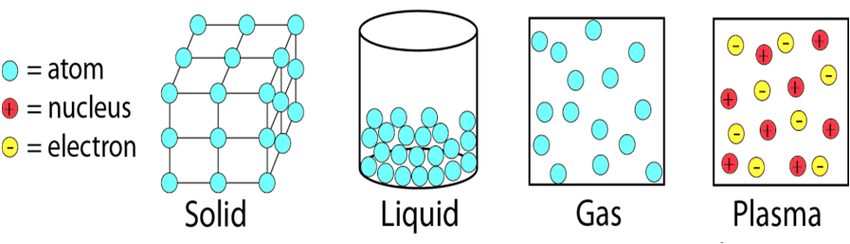
\includegraphics[scale=0.35]{imgs/plasma-graphic.png}

\end{frame}

\begin{frame}

\frametitle{What is fusion?}
\begin{columns}[T]

    \begin{column}{.5\textwidth}
        \begin{itemize}
            \item Abundant process in nature - see stars
            \item Large amounts of energy released
            \item Occurs most easily in plasma
        \end{itemize}
    \end{column}
    \vline\hspace{1em}

    \begin{column}{.5\textwidth}
        $$\prescript{2}{}{\text{H}} + \prescript{3}{}{\text{H}} \stackrel{\text{(fusion)}}{\to} \prescript{4}{}{\text{He}} + n + 17.59\;\text{MeV}$$
    \end{column}

\end{columns}

\end{frame}











\begin{frame}
\frametitle{What is a fusion reactor?}

\begin{columns}[T]

    \begin{column}{.5\textwidth}
        \textbf{What is it?}
        \begin{itemize}
            \item Controlled fusion for power generation
            \item Axisymmetric donut (spherical cow)
        \end{itemize}

        \textbf{Challenges}
        \begin{itemize}
            \item Confinement
            \item Runaway Electrons
            \item Sustaining the reaction
        \end{itemize}
    \end{column}

    \begin{column}{.5\textwidth}
        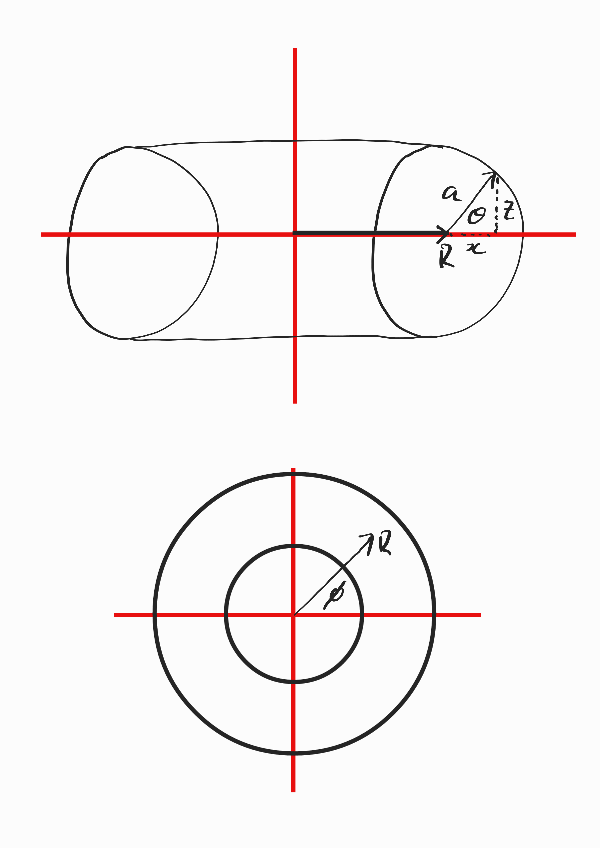
\includegraphics[scale=0.28]{imgs/dimensions.png}
    \end{column}

\end{columns}

\end{frame}













\begin{frame}
\frametitle{What is a fusion reactor?}

\begin{columns}[T]

    \begin{column}{.5\textwidth}
        \textbf{What is it?}
        \begin{itemize}
            \item Controlled fusion for power generation
            \item Axisymmetric donut (spherical cow)
        \end{itemize}

        \textbf{Challenges}
        \begin{itemize}
            \item \textcolor{red}{Confinement}
            \item \textcolor{red}{Runaway Electrons}
            \item Sustaining the reaction
        \end{itemize}
    \end{column}

    \begin{column}{.5\textwidth}
        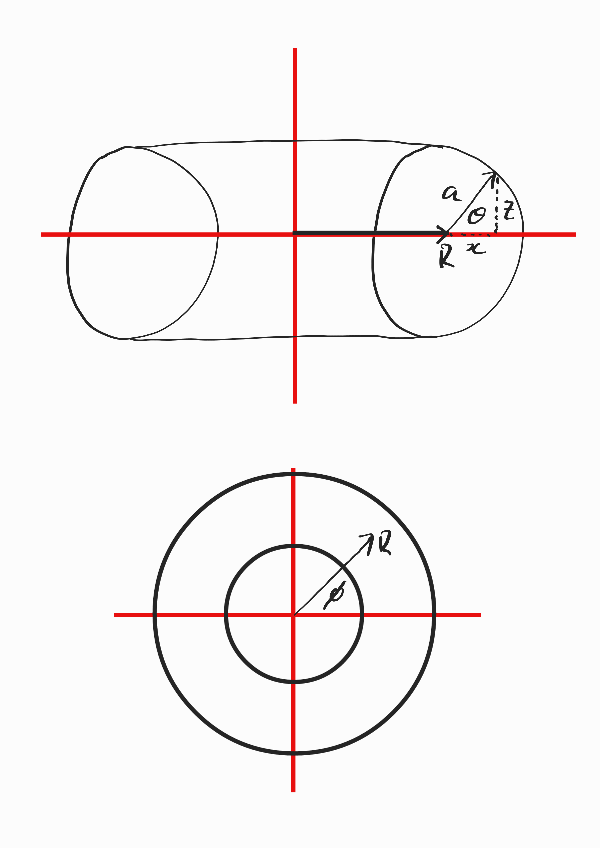
\includegraphics[scale=0.28]{imgs/dimensions.png}
    \end{column}

\end{columns}

\end{frame}
















\begin{frame}
\frametitle{What is a fusion reactor?}

\begin{columns}[T]

    \begin{column}{.5\textwidth}
        \textbf{What is it?}
        \begin{itemize}
            \item Controlled fusion for power generation
            \item Axisymmetric donut (spherical cow)
        \end{itemize}

        \textbf{Challenges}
        \begin{itemize}
            \item \textcolor{red}{Confinement}
            \item \textcolor{red}{Runaway Electrons}
            \item Sustaining the reaction
        \end{itemize}\vspace{9em}
    \end{column}

    \begin{column}{.5\textwidth}
        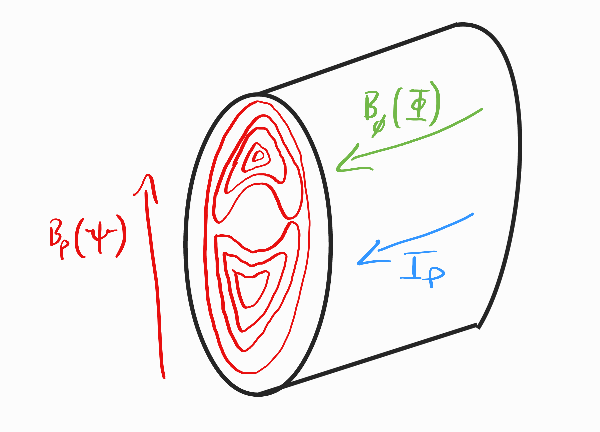
\includegraphics[scale=1.2]{imgs/flux-functions.png}
    \end{column}

\end{columns}

\end{frame}























\begin{frame}
\frametitle{What is an AC Tokamak?}

\begin{columns}[T]

    \begin{column}{.5\textwidth}
        \textbf{What is it?}
        \begin{itemize}
            \item Plasma current oscillates back and forth (AC)
            \item ISTTOK reactor (Artur in Portugal)
        \end{itemize}

        \textbf{Challenges?}
        \begin{itemize}
            \item Residual current density at $I_p = 0$
            \item Runaway electron population increase
        \end{itemize}
    \end{column}

    \begin{column}{.5\textwidth}
        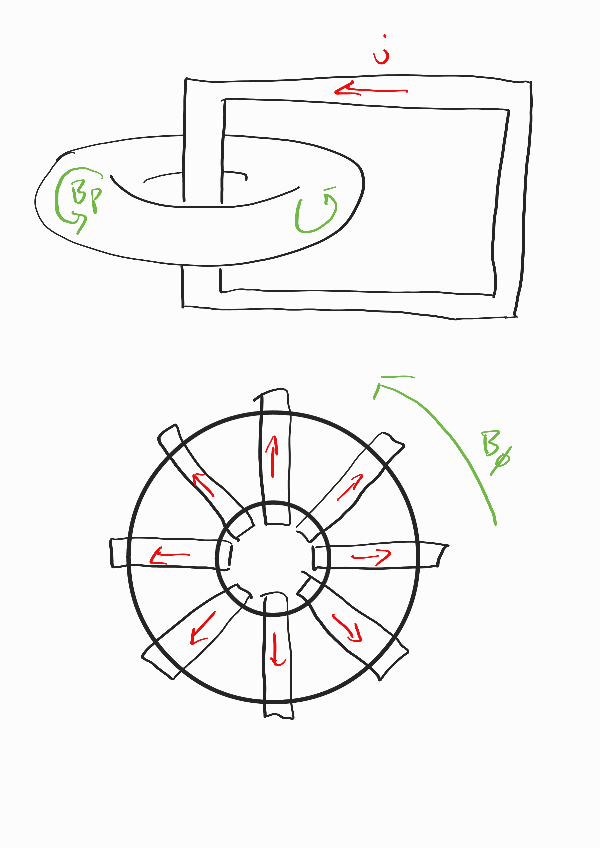
\includegraphics[scale=0.28]{imgs/solenoids.png}
    \end{column}

\end{columns}

\end{frame}














\begin{frame}
\frametitle{So what's the problem?}

\centering
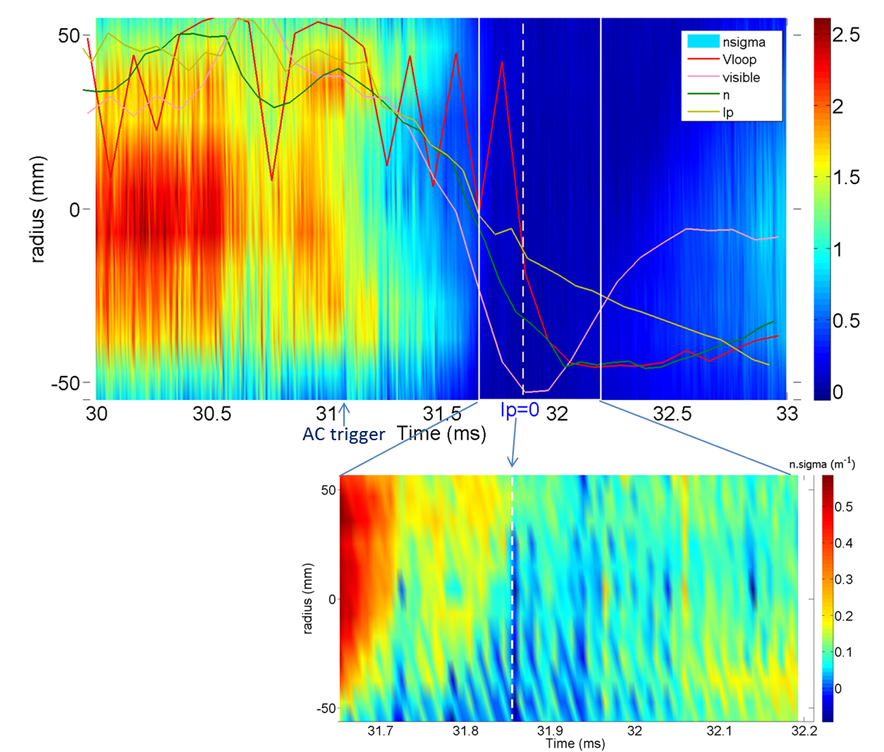
\includegraphics[scale=0.7]{imgs/residual-plasma.png}

\end{frame}

\begin{frame}
\frametitle{So what's the problem?}

\centering
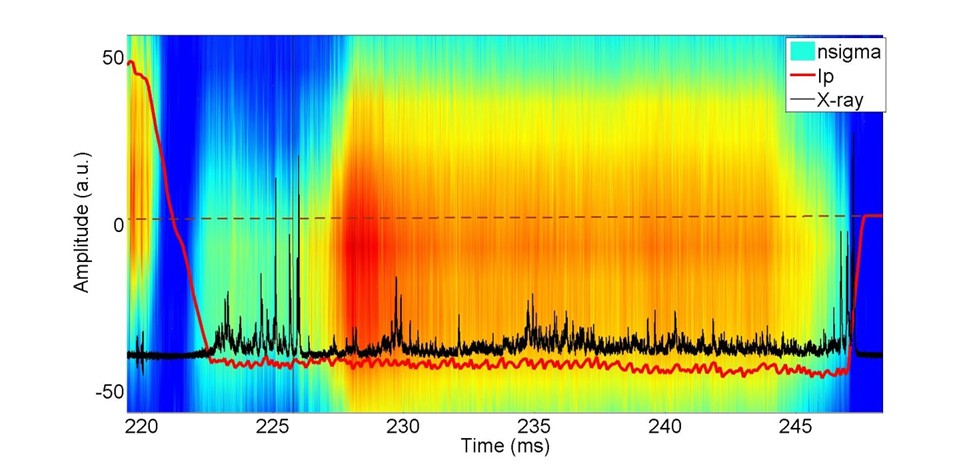
\includegraphics[scale=0.78]{imgs/re-presence.png}

\end{frame}













% Where should I introduce AC reactors? Talk about Artur and Matthew's work?




% FROM HERE:
% 2. Plasma Background
\begin{frame}
\frametitle{Modelling Plasma}

    \begin{columns}[T]
        \begin{column}{.5\textwidth}
            \textbf{Fluid Dynamics}
            \begin{align*}
                \pdv{\rho}{t} &= -\nabla \cdot (\rho \vec{u}) \\
                \rho \frac{\DD}{\DD t} \vec{u} &= \vec{F}
            \end{align*}
        \end{column}

        \begin{column}{.5\textwidth}
            \textbf{Maxwell's Equations}
            \begin{align*}
                \nabla \times \vec{B} &= \mu_0 \vec{j} + \frac{1}{c^2} \pdv{\vec{E}}{t} \\
                \nabla \times \vec{E} &= -\pdv{\vec{B}}{t} \\
                \nabla \cdot \vec{B} &= 0 \\
                \nabla \cdot \vec{E} &= \frac{\rho_c}{\epsilon_0}
            \end{align*}
        \end{column}
    \end{columns}

    \begin{center}
        \textbf{? MHD Equations ?}
    \end{center}

\end{frame}










\begin{frame}
\frametitle{Modelling Plasma}


    \textbf{MHD Equations}
    \begin{align*}
        \frac{\DD}{\DD t} \rho &= \rho \nabla \cdot \vec{u} \\
        \rho \frac{\DD}{\DD \vec{u}} &= -\nabla p + \vec{j} \times \vec{B} + \nabla \cdot \vec{\Pi} \\
        \frac{\DD}{\DD t} p &= -\gamma p \nabla \cdot \vec{u} + (\gamma - 1) \left [ -\nabla \cdot \vec{q} + \vec{\Pi} : \nabla \vec{u} + \eta j^2 \right ] \\
        \pdv{\vec{B}}{t} &= -\nabla \times \vec{E} \\
        \mu_0 \vec{j} &= \nabla \times \vec{B} \\
        \vec{E} + \vec{u} \times \vec{B} &= \eta \vec{j}
    \end{align*}

\end{frame}













\begin{frame}
\frametitle{Modelling Plasma}

\begin{columns}[T]

    \begin{column}{.5\textwidth}
        \textbf{Too cumbersome... Ideal MHD!}
        \begin{itemize}
            \item Resistivity is negligible
            \item No external source of heat / energy
            \item No extra source of pressure (e.g. gravitational)
        \end{itemize}
    \end{column}

    \begin{column}{.5\textwidth}
        \begin{align*}
            \frac{\DD}{\DD t} \rho &= \rho \nabla \cdot \vec{u} \\
            \rho \frac{\DD}{\DD \vec{u}} &= -\nabla p + \vec{j} \times \vec{B} \\
            \frac{\DD}{\DD t} p &= -\gamma p \nabla \cdot \vec{u} \\
            \pdv{\vec{B}}{t} &= -\nabla \times \vec{E} \\
            \mu_0 \vec{j} &= \nabla \times \vec{B} \\
            \vec{E} + \vec{u} &\times \vec{B} = 0
        \end{align*}
    \end{column}

\end{columns}
\end{frame}










\begin{frame}
\frametitle{Grad-Shafranov Equation}

\textbf{Assumptions}
\begin{itemize}
    \item Ideal MHD
    \item Axisymmetry
    \item Magnetic field topology fixed with respect to fluid (frozen-in flux condition)
\end{itemize}

\begin{equation*}
    x \pdv{x} \left ( \frac{1}{x} \pdv{\Psi}{x} \right ) + \pdv[2]{\Psi}{z} = -\mu_0 x^2 \pdv{p}{\Psi} - \mu_0^2 f(\Psi)\pdv{f}{\Psi}
\end{equation*}

$f(\Psi)$ is poloidal current density flux function; $p(\Psi)$ is pressure density flux function; and $\Psi(x,z)$ is the poloidal 
magnetic flux function.

\end{frame}















\begin{frame}
\frametitle{Grad-Shafranov-Helmholtz Equation}

\textbf{Notes}
\begin{itemize}
    \item Introduced by Wang
    \item Allows for current reversals
    \item Introduces $(a_1, a_2, \alpha)$
\end{itemize}

\begin{align*}
   \left ( x \pdv{x} \frac{1}{x} \pdv{x} + \pdv[2]{z} \right ) \psi &= -\frac{1}{2} x^2 \pdv{\beta}{\psi} - \frac{1}{2} \pdv{g^2}{\psi} = -xj_{\phi} \\
   -\frac{1}{2}\pdv{\beta}{\psi} &= a_1 \\
   -\frac{1}{2}\pdv{g^2}{\psi} &= -a_2 - \alpha^2 \psi (x, z)
\end{align*}

Oh also, has analytic solution! Boils down from an eigenvalue problem.

\end{frame}




















\begin{frame}
\frametitle{Grad-Shafranov-Helmholtz Equation}

\textbf{Solution}
\begin{equation*}
    \psi(x,z) = x \sum_{n = 1}^{\infty} \sum_{l = 0}^{\infty} \frac{(-1)^l 2 a_n^u}{kv_la_n^d (\alpha^2 - \lambda_{n,l}^2)} \left [ c_n J_1(\mu_n x) + N_1(\mu_n x)\right ] \cos(v_l z)
\end{equation*}
to go alongside
\begin{align*}
    \beta(x, z) &= \beta_0 - 2a_1 \psi(x, z) \\
    j_{\phi}(x,z) &= -a_1 x + \frac{1}{x} a_2 + \frac{\alpha^2}{x} \psi(x, z)
\end{align*}

Now have:
\begin{itemize}
    \item Poloidal magnetic flux 
    \item Current density
    \item Pressure density
\end{itemize}

\end{frame}














\begin{frame}
\frametitle{Wang Reproduction}

\centering
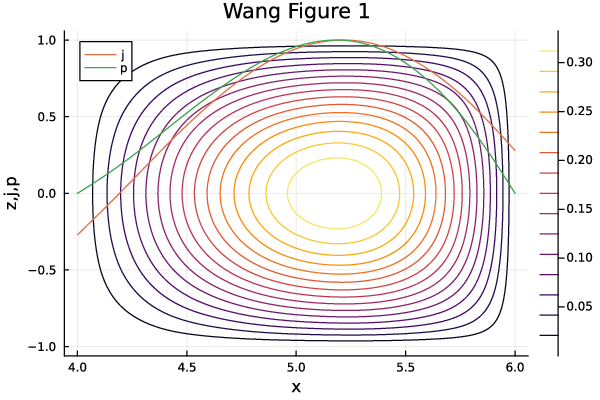
\includegraphics[scale=0.5]{imgs/wang-fig-1.png}

\end{frame}



\begin{frame}
\frametitle{Wang Reproduction}

\centering
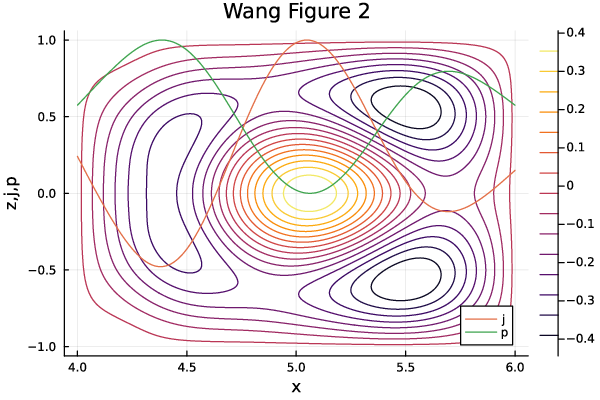
\includegraphics[scale=0.5]{imgs/wang-fig-2.png}

\end{frame}










\begin{frame}
\frametitle{Awesome}

Achievement get: reproduce figures\\ \vspace{3em}
Achievement not (yet) getted: animate figures \vspace{7em}


\end{frame}


\begin{frame}
\frametitle{Awesome}

Achievement get: reproduce figures\\ \vspace{3em}
Achievement not (yet) getted: animate figures \vspace{1em}

\textbf{Data Fitting}
\begin{itemize}
    \item Currently just specify $(a_1, a_2, \alpha)$
    \item Want to input data and get those values
    \item Least squares data fitting time
\end{itemize}

\end{frame}














\begin{frame}
\frametitle{Uh oh}

\centering
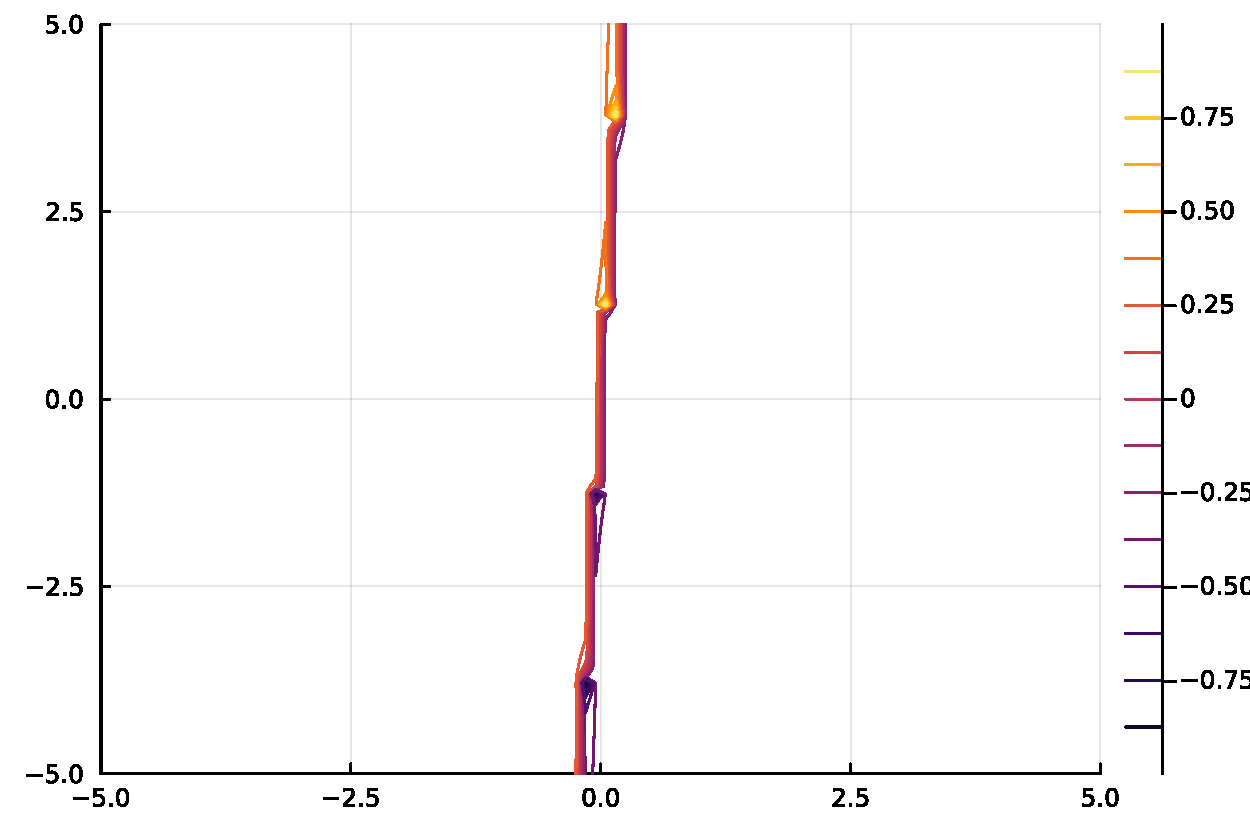
\includegraphics[scale=0.5]{imgs/what-1.pdf}

\end{frame}

\begin{frame}
\frametitle{Uh oh}

\centering
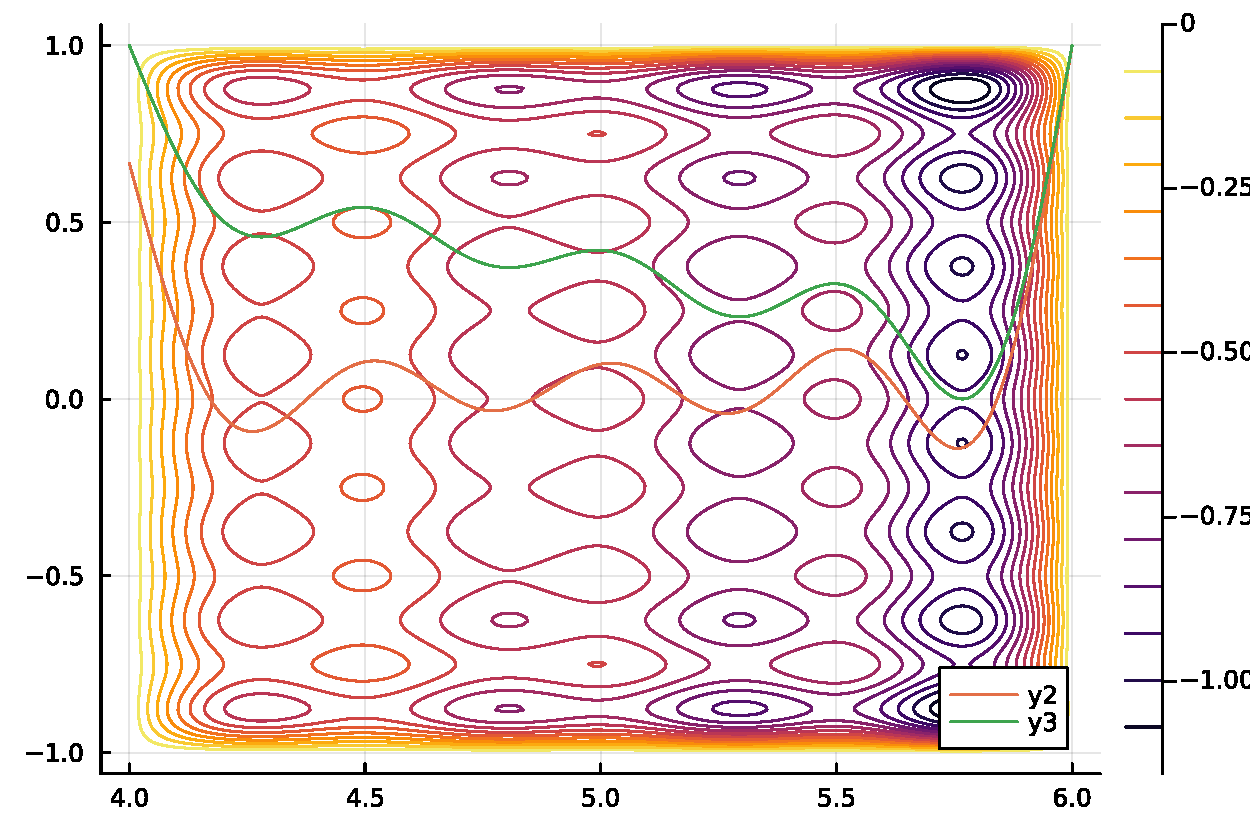
\includegraphics[scale=0.5]{imgs/what-2.pdf}

\end{frame}








\begin{frame}
\frametitle{What's going on?}


\centering
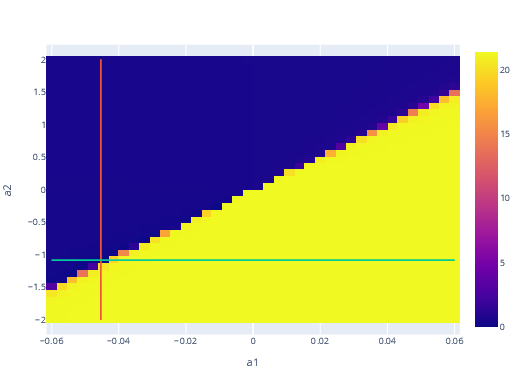
\includegraphics[scale=0.65]{imgs/heat-1-entire.png}


\end{frame}
    










\begin{frame}
\frametitle{How fix?}

\begin{itemize}
    \item Include more data (using current density... could add pressure?)
    \item Use a different model?
    \item Use a different optimisation method?
    \item Modify our optimisation approach?
\end{itemize}\vspace{6em}
\end{frame}

\begin{frame}
\frametitle{How fix?}

\begin{itemize}
    \item Include more data (using current density... could add pressure?)
    \item Use a different model?
    \item Use a different optimisation method?
    \item Modify our optimisation approach?
\end{itemize}

\textbf{Now:}
\begin{itemize}
    \item Provide initial guess which is ``close to'' actual $(a_1, a_2, \alpha)$
    \item Works! (we've just replicated the Wang figure again, but with data instead)
\end{itemize}
\end{frame}

\begin{frame}
\frametitle{Simulated}

\centering
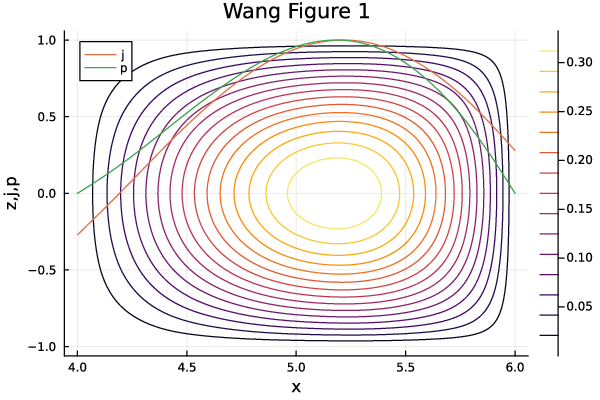
\includegraphics[scale=0.5]{imgs/wang-fig-1.png}

\end{frame}












\begin{frame}
\frametitle{Current Inversion}

\textbf{Goal:}
\begin{itemize}
    \item Simulate quiescent phase of current reversal
    \item Observe magnetic field topology changes
    \item Pressure density effects
    \item Do this using data (foreshadowing ISTTOK)
\end{itemize}
\textbf{How:}
\begin{itemize}
    \item Solve for $(a_1, a_2, \alpha)$ in successive equilibrium time slices
    \item Use solution of one to feed in as initial guess for next
    \item Question: what do we use as a guess for first time slice?
\end{itemize}
\end{frame}









\begin{frame}
\frametitle{Simulated Reversal}

If you're seeing this, something has gone wrong... General Kenobi.

\textcolor{red}{DONT FORGET TO PUT ANIMATION HERE}

\end{frame}

\begin{frame}
\frametitle{Simulated Reversal}

If you're seeing this, something has gone wrong... General Kenobi.

\textcolor{red}{DONT FORGET TO PUT ANIMATION HERE}

\end{frame}

\begin{frame}
\frametitle{Simulated Quiescent Reversal}

If you're seeing this, something has gone wrong... General Kenobi.

\textcolor{red}{DONT FORGET TO PUT ANIMATION HERE}

\end{frame}

\begin{frame}
\frametitle{Simulated Quiescent Reversal}

If you're seeing this, something has gone wrong... General Kenobi.

\textcolor{red}{DONT FORGET TO PUT ANIMATION HERE}

\end{frame}
    








\begin{frame}
\frametitle{ISTTOK Data}
\begin{itemize}
    \item Current density profile, pressure density profile, $v_{\text{loop}}$
    \item Use current density to get $(a_1, a_2, \alpha)$
    \item Compare simulated density profiles to data for accuracy of model
    \item \dots 
    \item Profit?
\end{itemize}
\end{frame}


\begin{frame}
\frametitle{Initial ISTTOK Simulation}

    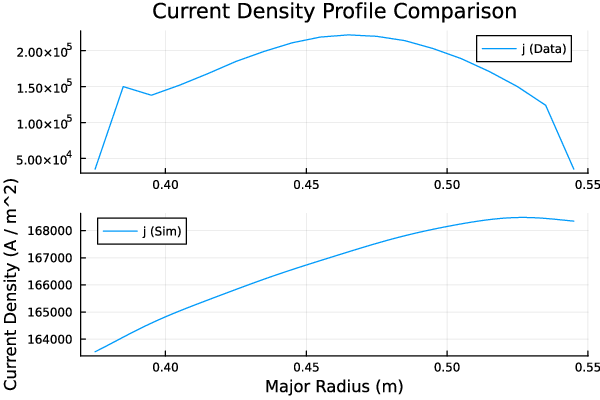
\includegraphics[scale=0.5]{imgs/comparison-current-0-unfiltered.png}

\end{frame}


\begin{frame}
\frametitle{Scientific Creative Liberty Simulations}

    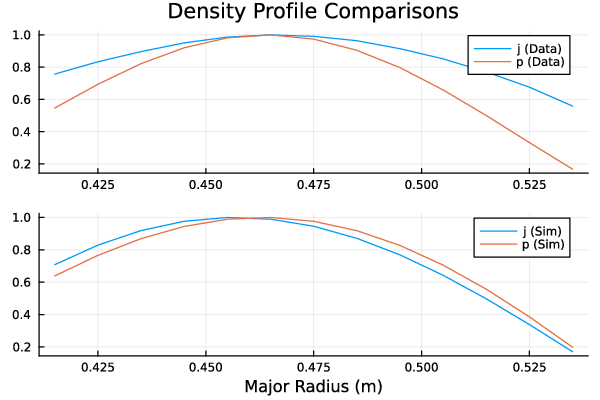
\includegraphics[scale=0.5]{imgs/comparison-cp-edited-0.png}
\end{frame}


\begin{frame}
\frametitle{ISTTOK Magnetic Field Topology}

    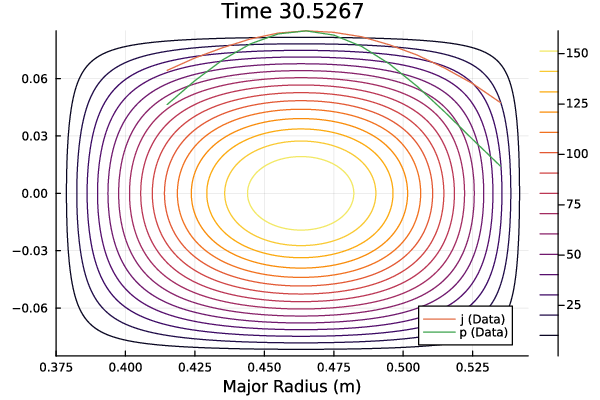
\includegraphics[scale=0.55]{imgs/mag-field-edited-data-0.png}

\end{frame}



\begin{frame}
\frametitle{The Other Time Slices?}

    \begin{itemize}
        \item Model struggles to converge - highly parameter sensitive
        \item Data quite imprecise - manual manipulation to achieve above
        \item Still question of first time slice's parameter guess 
        \item Combine what we can model with other simulations (work with Artur)
    \end{itemize}
    \textbf{Further Work}
    \begin{itemize}
        \item Data interpolation methods (inter- and intra- time slice)
        \item Electric field information (helpful for REs)
        \item Inclusion of pressure density profile in fitting (compare $v_{\text{loop}}$ instead)
    \end{itemize}
\end{frame}












\begin{frame}
\frametitle{(BONUS) Cool Ion Diagnostics}

    \centering
    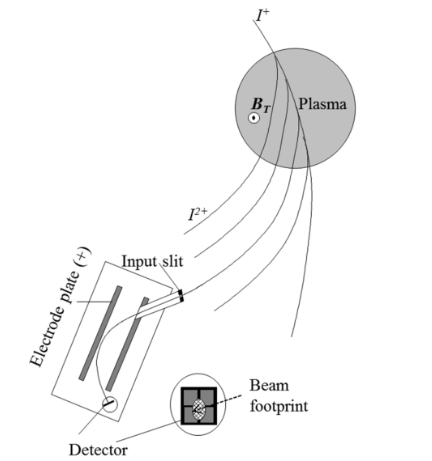
\includegraphics[scale=0.6]{imgs/ion-diagnostics.png}

\end{frame}
\end{document}